\documentclass[11pt]{article}
\usepackage[utf8]{inputenc}
\usepackage[T1]{fontenc}
\usepackage{grffile}
\usepackage{longtable}
\usepackage{wrapfig}
\usepackage{rotating}
\usepackage[normalem]{ulem}
\usepackage{amsmath}
\usepackage{textcomp}
\usepackage{amssymb}
\usepackage{multirow}
\usepackage{capt-of}
\usepackage{hyperref}
\hypersetup{colorlinks=true, linkcolor=magenta}
\setlength{\parindent}{0in}
\usepackage[margin=1in]{geometry}
\usepackage[spanish]{babel}
\usepackage{mathtools}
\usepackage{palatino}
\usepackage{fancyhdr}
\usepackage{sectsty}
\usepackage{engord}
\usepackage{parskip}
\usepackage{minted}
\usepackage{cite}
\usepackage{graphicx}
\usepackage{subcaption}
\usepackage{setspace}
\usepackage[compact]{titlesec}
\usepackage[center]{caption}
\usepackage{placeins}
\usepackage{color}
\usepackage{amsmath}
\usepackage{varwidth}
\usepackage{bm}
\usepackage{todonotes}
\usepackage{pdfpages}
% \titlespacing*{\subsection}{0pt}{5.5ex}{3.3ex}
% \titlespacing*{\section}{0pt}{5.5ex}{1ex}
\decimalpoint
\author{Antonio Coín Castro}
\date{\today}
\title{Procesamiento de Información Temporal\\\Large{Práctica 2}}
\hypersetup{
 pdfauthor={Antonio Coín Castro},
 pdftitle={},
 pdfkeywords={},
 pdfsubject={},
 pdflang={Spanish}}

\begin{document}

\maketitle

\section{Modificando la configuración y arquitectura del VAD basado en LSTM}

\subsection{Validación (evaluación) del modelo de la práctica 1}

\textbf{Pregunta 1.} \textit{Incluya en la memoria de la práctica el código utilizado, incluyendo los valores de cualquier parámetro de configuración utilizado (por ejemplo, el número de épocas de entrenamiento realizadas).}

\textit{Respuesta}. Para entrenar y validar el modelo, dividimos el código en tres funciones. La primera de ella encapsula el comportamiento de una época de entrenamiento, muy similar a la desarrollada en la práctica anterior. Nos servimos también de las funciones \texttt{get\_feat} y \texttt{get\_lab} de la práctica anterior para ir creando los \textit{batches} de datos. Notamos que además hemos añadido la opción de codificar las etiquetas para una hipotética salida con dos neuronas y activación softmax (se usa en los modelos de la Sección \ref{sec:2}).

\begin{minted}{python}
from keras.utils.np_utils import to_categorical

def train_for_epoch(segment_sets, n_features):
  model.train()
  cache_loss = 0.0
  cache_acc = 0.0
  n_elems = 0

  # Loop through batches
  for segment_set in segment_sets:
    rand_idx = {}
    optimizer.zero_grad()

    # Create training batches
    feats_batch = np.vstack(
      [get_feat(TRAIN_PATH + segment, rand_idx, n_features)
       for segment in segment_set])
    if SOFTMAX_ENCODING:
      labs_batch = np.vstack(
        [to_categorical(
          get_lab(TRAIN_PATH + segment, rand_idx),
          num_classes=2).astype(np.int16)
         for segment in segment_set])
    else:
      labs_batch = np.vstack(
        [get_lab(TRAIN_PATH + segment, rand_idx).astype(np.int16)
         for segment in segment_set])

    # Shuffle the data and place them into Pytorch tensors
    shuffle = np.random.permutation(len(labs_batch))
    labs_batch = torch.tensor(
      labs_batch.take(shuffle, axis=0).astype("float32")).to(device)
    feats_batch = torch.tensor(
      feats_batch.take(shuffle, axis=0).astype("float32")).to(device)

    # Forward the data through the network
    predictions = model(feats_batch)
    # Compute cost
    loss = criterion(predictions, labs_batch)
    # Backward step
    loss.backward()
    optimizer.step()

    # Save stats
    cache_loss += loss.item()
    if SOFTMAX_ENCODING:
      cache_acc += (torch.eq(
      torch.argmax(predictions, dim=2),
      torch.argmax(labs_batch, dim=2))).sum()
    else:
      cache_acc += (torch.eq(predictions >= 0.5, labs_batch)).sum()
    n_elems += np.prod(predictions.shape[:2])

  epoch_loss = cache_loss/len(segment_sets)
  epoch_acc = cache_acc/n_elems
  return epoch_loss, epoch_acc.cpu()
\end{minted}

La función para validar es similar, cambiando simplemente la ruta de donde sacamos los datos, y eliminando el \textit{backpropagation} y los pasos del optimizador. Tan solo pasamos los datos hacia delante por la red y obtenemos las predicciones, la pérdida y el \textit{accuracy}.

\begin{minted}{python}
def validate(segment_sets, n_features):
  model.eval()
  cache_loss = 0.0
  cache_acc = 0.0
  n_elems = 0

  # We don't need gradients for validation
  with torch.no_grad():
    # Loop through batches
    for segment_set in segment_sets:
      rand_idx = {}

      # Create validation batches
      feats_batch = np.vstack(
        [get_feat(VALID_PATH + segment, rand_idx, n_features)
         for segment in segment_set])
      if SOFTMAX_ENCODING:
        labs_batch = np.vstack(
          [to_categorical(
            get_lab(VALID_PATH + segment, rand_idx),
            num_classes=2).astype(np.int16)
           for segment in segment_set])
      else:
        labs_batch = np.vstack(
          [get_lab(VALID_PATH + segment, rand_idx).astype(np.int16)
           for segment in segment_set])

      # Place data into Pytorch tensors (no shuffle!)
      labs_batch = torch.tensor(labs_batch.astype("float32")).to(device)
      feats_batch = torch.tensor(feats_batch.astype("float32")).to(device)

      # Forward the data through the network
      predictions = model(feats_batch)

      # Compute cost
      loss = criterion(predictions, labs_batch)

      # Save stats
      cache_loss += loss.item()
      if SOFTMAX_ENCODING:
        cache_acc += (torch.eq(
        torch.argmax(predictions, dim=2),
        torch.argmax(labs_batch, dim=2))).sum()
      else:
        cache_acc += (torch.eq(predictions >= 0.5, labs_batch)).sum()
      n_elems += np.prod(predictions.shape[:2])

    epoch_loss = cache_loss/len(segment_sets)
    epoch_acc = cache_acc/n_elems

  return epoch_loss, epoch_acc.cpu()
\end{minted}

Finalmente, creamos una función que itere sobre las épocas de entrenamiento y vaya mostrando por pantallas las estadísticas correspondientes.

\begin{minted}{python}
def train(first_epoch, num_epochs, n_features=20):
  train_losses, valid_losses, train_accs, valid_accs = [], [], [], []

  for epoch in range(first_epoch, first_epoch + num_epochs):
    # Training phase
    train_loss, train_acc = train_for_epoch(train_segments, n_features)

    # Validation phase
    valid_loss, valid_acc = validate(valid_segments, n_features)

    print(f'[{epoch:02d}] train loss: {train_loss:03f}  '
          f'val loss: {valid_loss:03f}  '
          f'train acc: {train_acc*100:.3f}%  '
          f'val acc: {valid_acc*100:.3f}%')

    train_losses.append(train_loss)
    valid_losses.append(valid_loss)
    train_accs.append(train_acc)
    valid_accs.append(valid_acc)

  return train_losses, valid_losses, train_accs, valid_accs
\end{minted}

Para configurar el entrenamiento, fijamos el número de épocas a 4 como en la práctica anterior, considerando como longitud de segmento 300 frames. Además, utilizamos el mismo modelo, el mismo optimizador (Adam con \textit{learning rate} de $10^{-3}$) y la misma función de pérdida que en la práctica 1. En cuanto al tamaño de \textit{batch}, mantenemos 51 en entrenamiento para que cada época haga exactamente 10 iteraciones, y establecemos el tamaño de batch en validación a 72, ya que solo disponemos de 72 audios de validación (así en cada época se recorren todos los datos en un solo \textit{batch}).

\textbf{Pregunta 2.} \textit{¿Qué rendimiento (loss y accuracy) obtiene con este modelo (Model\_1) en entrenamiento y en validación? }

\textit{Respuesta}. El rendimiento del modelo a lo largo de las épocas se puede observar en la Figura \ref{fig:1}, tanto en entrenamiento como en validación (al final de cada época).

\begin{figure}[h!]
  \centering
  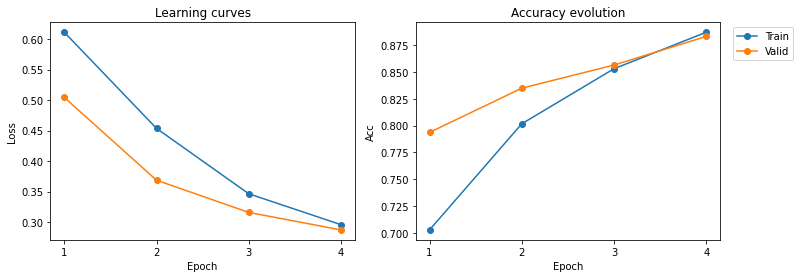
\includegraphics[width=\textwidth]{img/1_learning_curves}
  \caption{Pérdida y \textit{accuracy} del modelo en entrenamiento y validación.}
  \label{fig:1}
\end{figure}

Tras finalizar el entrenamiento obtenemos los siguientes resultados:
\newpage

\begin{table}[h!]
  \centering
  \begin{tabular}{c|cc}
     & Pérdida & \textit{Accuracy} (\%)\\
    \hline
    Entrenamiento & 0.2958 & 88.701\\
    Validación & 0.2872 & 88.310\\
  \end{tabular}
\end{table}

Como vemos, los resultados tanto en entrenamiento como en validación son similares, y se observa una tendencia decreciente en la pérdida y ascendente en el \textit{accuracy}. Esto quiere decir que el modelo está aprendiendo correctamente y que no hay \textit{overfitting}.

\subsection{Modificación de la longitud de la secuencia}

\textbf{Pregunta 3}. \textit{Describa brevemente cómo ha realizado la compensación de datos para poder comparar los modelos de una forma más justa.}

\textit{Respuesta}. La idea ha sido mantener aproximadamente constante la cantidad total de audio utilizada para entrenar el modelo, tanto en total como por cada fichero de audio. Para ello, modificamos el número de épocas para intentar compensar por la disminución o el aumento de la longitud de la secuencia. Sabemos que si 300 frames eran 3 segundos, 100 frames serán 1 segundo (aproximadamente). La cantidad total de frames de audio que considerábamos antes era:
$$
4 \text{ épocas} \cdot 510 \text{ ficheros} \cdot 300 \text{ frames} = 612000 \text{ frames}.
$$

Para compensar por usar secuencias de 1 segundo (3 veces más pequeñas), multiplicamos el número de épocas por 3, realizando un total de 12 épocas. Por otra parte, para compensar por usar secuencias de 30 segundos, deberíamos realizar 10 veces menos épocas, pero no podemos hacer menos de una época usando todos los datos. Es por esto que decidimos hacer 1 época de entrenamiento en este último caso.

\textbf{Pregunta 4.} \textit{¿Qué rendimiento obtiene para la red entrenada con secuencias de 1 segundo de longitud sobre el conjunto de validación? ¿Y para la de 30 segundos? Comente brevemente los motivos por los que esto puede ocurrir. }

\textit{Respuesta}. Podemos ver las curvas de entrenamiento y validación del modelo con secuencias de 1 segundo en la Figura \ref{fig:2}.

\begin{figure}[h!]
  \centering
  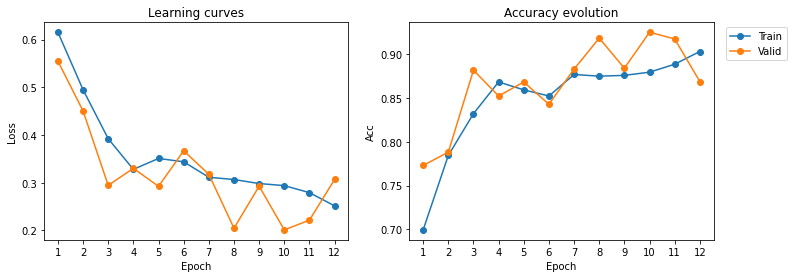
\includegraphics[width=\textwidth]{img/2_learning_curves}
  \caption{Pérdida y \textit{accuracy} del modelo con secuencias de 1 segundo en entrenamiento y validación.}
  \label{fig:2}
\end{figure}

Para longitud de secuencia de 30 segundos no tiene sentido hacer estas gráficas, ya que solo entrenamos durante una época. Una cosa a tener en cuenta para este modelo es que había audios cuya longitud era menor de 30 segundos, y tal y como estaba diseñado el código había fallos en la ejecución y no se podía entrenar. Para solucionar esto había, al menos, tres posibles enfoques:
\begin{itemize}
  \item Considerar secuencias de longitud dinámica, rellenando por ejemplo con 0s hasta completar los 30 segundos en aquellas señales con tamaño menor. Esto requeriría modificar el modelo y añadir capas que realicen algún tipo de \textit{masking} de las secuencias, para descartar en tiempo de ejecución aquellas partes que no sean realmente audio.
  \item Truncar todos los audios para que tengan como longitud el mínimo de las longitudes de todos ellos, o directamente ignorar aquellos que no lleguen a 30 segundos. Requeriría modificar los datos.
  \item Considerar un tamaño de \textit{batch} de 1 e ir pasando los audios individualmente al modelo. No requiere ningún cambio en el código salvo modificar el valor de la variable de \textit{batch\_size}.
\end{itemize}

Finalmente elegimos la tercera opción, por ser la más sencilla. La desventaja de hacer esto es que, al tener más pasos del optimizador (uno por cada audio en lugar de uno por cada \textit{batch}), el proceso no es tan comparable a los modelos anteriores, y además el entrenamiento se vuelve un poco más largo.

Los resultados numéricos para los tres modelos considerados hasta ahora, obtenidos tras la última época de entrenamiento en cada caso, son los siguientes:

\begin{table}[h!]
  \centering
  \begin{tabular}{c|ccc}
      & Longitud segmento (s) & Pérdida & \textit{Accuracy} (\%)\\
    \hline
    \multirow{3}{*}{Entrenamiento} & 1 & 0.2513   & 90.314\\
    & 3 & 0.2958 & 88.701\\
    &30 & 0.2751  & 88.714\\\hline
    \multirow{3}{*}{Validación} & 1 & 0.3067 & 86.889\\
    &  3 & 0.2872 & 88.310\\
   &30 & 0.2155 & 91.264\\
  \end{tabular}
\end{table}

Como vemos, los mejores resultados en entrenamiento se obtienen con segmentos de 1s, mientras que en validación el rendimiento es mejor con segmentos de 30s. Sin embargo, veíamos en la Figura \ref{fig:2} que los resultados fluctúan bastante (sobre todo en validación), por lo que tampoco podemos sacar conclusiones muy significativas sobre ellos. Algo que sí observamos es que todos los resultados se encuentran en un rango más o menos parecido, por lo que parece que la longitud de la secuencia no afecta demasiado al rendimiento. Esto tiene sentido, ya que hemos intentado compensar para tener la misma cantidad total de audio, y al estar usando redes recurrentes con memoria, estas aprenden a retener tan solo el contexto relevante en cada secuencia, llegando al final a buenos resultados en todos los casos.

\subsection{Redes bidireccionales LSTM}

\textbf{Pregunta 5.} \textit{Explique brevemente la diferencia entre una capa LSTM y una BLSTM (bidirectional LSTM).}

\textit{Respuesta}. Las redes LSTM bidireccionales son una extensión de las redes LSTM usuales. Están formadas por dos redes LSTM que se entrenan sobre la entrada original y sobre una copia de la entrada invertida (en orden inverso en el tiempo), respectivamente. De esta forma, se proporciona contexto adicional a la red (tanto pasado como futuro) que puede mejorar el rendimiento y la velocidad de aprendizaje.

\textbf{Pregunta 6.} \textit{Incluya el código donde define Model\_1B en el informe de la práctica.}

\textit{Respuesta}. Podemos ver el código a continuación. Tan solo tenemos que activar el parámetro \texttt{bidirectional} de la capa LSTM.

\begin{minted}{Python}
class Model_1B(nn.Module):
  def __init__(self, feat_dim=20):
    super(Model_1B, self).__init__()
    self.lstm = nn.LSTM(
      feat_dim, 256, batch_first=True, bidirectional=True)
    self.output = nn.Linear(2*256, 1)

  def forward(self, x):
    out = self.lstm(x)[0]
    out = self.output(out)
    out = torch.sigmoid(out)
    return out.squeeze(-1)
\end{minted}

\textbf{Pregunta 7.} \textit{¿Qué modelo obtiene un mejor resultado sobre los datos de validación para las secuencias de 3 segundos? ¿Por qué puede ocurrir esto?}

\textit{Respuesta}. Para los datos de validación, el modelo \textit{Model\_1} con secuencias de 3 segundos obtiene un \textit{accuracy} de $88.31\%$, como vimos antes. El modelo \textit{Model\_1B}, por su parte, obtiene un \textit{accuracy} de validación de $91.62\%$ con el mismo número de épocas y la misma longitud de segmento. Como vemos el resultado es mejor en el nuevo modelo. Esto puede ocurrir porque, como hemos comentado, el hecho de aumentar el contexto y entrenar una red con la entrada y otra con la entrada invertida puede hacer que se aprenda más rápido y mejor, necesitando menos épocas para obtener los mismos resultados.

\textbf{Pregunta 8.} \textit{¿Y para las secuencias de 1 segundo? ¿Por qué?}

En el caso de secuencias de 1 segundo obteníamos con el modelo \textit{Model\_1} un \textit{accuracy} en validación de $86.89\%$, mientras que con el modelo \textit{Model\_1B} obtenemos un $94\%$. De nuevo, esta mejora se debe al contexto temporal adicional que tiene la red, pues está viendo ``a la vez'' como se comporta la señal hacia delante y hacia atrás en el tiempo, lo que hace que el aprendizaje y la generalización sean mejores.

\subsection{Modelo más profundo}

\textbf{Pregunta 9.} \textit{Incluya el código de la clase Model\_2 en la memoria.}

\textit{Respuesta}. En este caso aumentamos el parámetro \texttt{num\_layers} de la capa LSTM a 2.

\begin{minted}{Python}
class Model_2(nn.Module):
  def __init__(self, feat_dim=20):
    super(Model_2, self).__init__()
    self.lstm = nn.LSTM(
        feat_dim, 256, num_layers=2,
        batch_first=True, bidirectional=False)
    self.output = nn.Linear(256, 1)

  def forward(self, x):
    out = self.lstm(x)[0]
    out = self.output(out)
    out = torch.sigmoid(out)
    return out.squeeze(-1)
\end{minted}

\textbf{Pregunta 10}. \textit{¿Qué modelo obtiene un mejor resultado sobre los datos de validación, Model\_1 o Model\_2? ¿Por qué puede ocurrir esto?}

\textit{Respuesta}. En este caso, con Model\_2 se obtiene un \textit{accuracy} en validación del $88.85\%$, muy similar al el que obteníamos con el modelo Model\_1, que recordemos era de $88.31$. Parece ser que en este caso el hecho de tener más capas no ha surtido mucho efecto, pues la red ya estaba aprendiendo adecuadamente con una única capa. Además, al haber incrementado el número de parámetros por meter una nueva capa, estamos haciendo que potencialmente se necesite más tiempo de entrenamiento para ajustar correctamente los pesos, pudiendo llegar incluso a caer en \textit{overfitting} si no disponemos de demasiados ejemplos de entrenamiento.

\textbf{Pregunta 11}. \textit{¿Y con respecto a Model\_1B, cuál es mejor?}

\textit{Respuesta}. Model\_2 sale perdiendo frente a Model\_1B, pues este último llegaba a alcanzar un \textit{accuracy} en validación de $91.62\%$, frente al $88.85$ de Model\_2. Esto parece reforzar la hipótesis de que añadir otra capa extra de la misma dimensión no es la mejor decisión para aumentar el rendimiento con nuestros datos. Podríamos argumentar que es mejor desde un punto de vista de eficiencia y aprendizaje proporcionar un contexto extra a la red mediante una capa bidireccional. Aunque esta última es también en esencia un modelo con dos capas LSTM, al invertir la entrada en una de ellas hacemos que sea ``diferente'' y más útil en el modelo.

\section{Convolutional DNN + LSTM}
\label{sec:2}

\subsection{Modelo CDNN}

\textbf{Pregunta 12.} \textit{Incluya el código de la clase Model\_CDNN}.

\textit{Respuesta}. La idea de este modelo es interpretar las características Mel de un audio para una discretización de tiempo como una matriz (una ``imagen'' con un único canal), y realizar sobre ella una convolución en frecuencia antes de pasarla a un modelo de LSTM similar al que construíamos en los ejercicios anteriores. El código se puede ver a continuación:

\begin{minted}{Python}
class Model_CDNN(nn.Module):
  def __init__(self, P=40, freq_conv_filters=32, n_lstm=1, n_cells=32):
    super(Model_CDNN, self).__init__()
    self.freqConv = nn.Sequential(
      # Convolution along the frequency axis (batch_size, 1, seq_length, P)
      nn.Conv2d(1, freq_conv_filters, kernel_size=(1, 8)),
      nn.MaxPool2d(kernel_size=(1, 3)),  # non-overlapping by default
      nn.ReLU(inplace=True)
    )
    freqConv_output = int((P - 8 + 1)/3)
    self.lstm = nn.LSTM(freq_conv_filters*freqConv_output, n_cells,
                        batch_first=True, bidirectional=False,
                        num_layers=n_lstm)
    self.output = nn.Linear(n_cells, 2)

  def forward(self, x):
    """Expected input is (batch_size, seq_length, P)"""
    x_channels = x.unsqueeze(1) # -> (batch_size, 1, seq_length, P)
    out = self.freqConv(x_channels)

    # Flatten frequency values across all channels
    out = out.permute(0, 2, 1, 3)
    out = out.reshape(x.shape[0], x.shape[1], -1)

    out = self.lstm(out)[0]
    out = self.output(out)
    out = nn.Softmax(dim=2)(out)

    return out
\end{minted}

Algunos detalles a tener en cuenta son:
\begin{itemize}
  \item Hay que tener cuidado con el formato de entrada de los datos. La capa convolucional espera un \textit{shape} de (batch\_size, 1, seq\_length, 40), donde el 1 simboliza los canales de la ``imagen''. Sin embargo, para facilitar las cosas añadimos esta dimensión extra dentro del propio modelo, así que no es necesario modificar el formato de entrada respecto al modelo de ejercicios anteriores.
  \item Para tomar la salida de la convolución como entrada de la LSTM necesitamos perder una dimensión, ya que ahora nuestra ``imagen'' pasa a tener más de un canal (por defecto 32). Lo más razonable es concatenar en cada posición de la dimensión de la frecuencia los valores de todos los canales resultantes. Esto lo materializamos en la función \texttt{forward} mediante un \texttt{reshape} adecuado.
  \item El modelo está definido con dos neuronas de salida y activación softmax. Debemos obtener las etiquetas en formato adecuado, usando one-hot encoding. Si activamos este parámetro, podemos reutilizar las mismas funciones de entrenamiento y validación de la Pregunta 1 para probar el modelo, usando 40 características (las 20 MFCC y sus primeras derivadas, por ejemplo).
\end{itemize}


\subsection{Modelo Raw Waveform CDNN}

\textbf{Pregunta 13.} \textit{Incluya el código de la clase Model\_CDNN\_raw}.

\textit{Respuesta}. El nuevo modelo se ha enfocado desde el punto de vista de la implementación como una clase que hereda del modelo CDNN.

\begin{minted}{Python}
class Model_CDNN_raw(Model_CDNN):
  def __init__(self, P=40, N=401, freq_conv_filters=16,
               n_lstm=2, n_cells=16):
    super(Model_CDNN_raw, self).__init__(
      P, freq_conv_filters, n_lstm, n_cells)
    # Expected input is (batch_size, 1, n_samples)
    self.P = P
    self.timeConv = nn.Sequential(
      nn.Conv1d(1, P, kernel_size=N),
      nn.AdaptiveMaxPool2d(output_size=(None, 1))
    )

  def forward(self, x):
    """Expected input is (batch_size, seq_length, n_samples)"""
    out = np.zeros((x.shape[0], x.shape[1], self.P))
    out = x.new_tensor(out)  # (batch_size, seq_length, P)

    for i in range(x.shape[1]):
      seq = x[:, i, :].unsqueeze(1)  # (batch_size, 1, n_samples)
      freq_features = self.timeConv(seq).squeeze(-1)
      out[:, i] = torch.log(F.relu(freq_features) + 0.01)  # stabilized log
    out = super().forward(out)

    return out
\end{minted}

En primer lugar se realiza una convolución en el tiempo de la señal original, para obtener un vector P-dimensional por cada frame. Este procedimiento se realiza por cada fragmento de la señal que tengamos (que se han obtenido previamente con ventanas solapadas, por ejemplo cada 10ms), y después se concatenan los resultados para obtener una matriz que se pasa como entrada al modelo CDNN.

\end{document}
